\chapter{Data Reduction}
\label{cha:dataReduction}
\section{Calibration}
To actually calibrate the detectors, we use an $\alpha$-source with a known spectrum. The source is placed in the target position, and each detector is in turn placed in front of the source. 
The radioactive source used to calibrate this setup contained \isotope[148][]{Gd}, \isotope[239][]{Pu} and \isotope[244][]{Cm}. Each isotope has a prominent main peak, and several sub peaks. The proprieties of which is listed in  \cref{tab:cali}.
\begin{table}[H]
	\centering
	\begin{tabular}{ll}
		Isotope & $E_\alpha \ [keV]$  \\ \hline
		\isotope[148][]{Gd}		& 3182.690         \\
		\isotope[239][]{Pu}		& 5105.5           \\
								& 5144.3           \\
								& 5156.59          \\
		\isotope[244][]{Cm}		& 5762.64          \\
								& 5804.96          \\ 
	\end{tabular}
	\caption{Decay energies for each isotope used in the calibration.}
	\label{tab:cali}
\end{table}
A typical single strip spectrum is shown on \cref{fig:singleStripExample}, where the calibrator has given an estimate of where the peaks are, illustrated by the red triangles. \cref{fig:peakExample} shows a closer look at the \isotope[244][]{Cm} peak, where the red line shows the \texttt{Calibrator}-fit over both the main peak and the sub peak. \\

\begin{figure}[H]
	\begin{subfigure}{\linewidth}
		\centering
		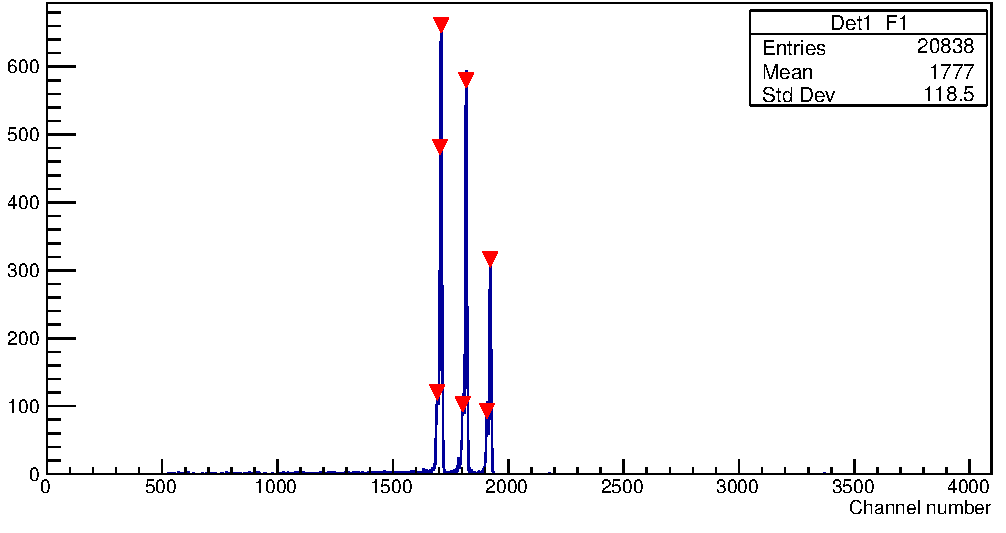
\includegraphics[width=.9\linewidth]{../figures/cali/det1f1-cropped.pdf}
		\caption{A spectrum of the calibration source, with channel number along the x-axis. The red triangles indicate the positions the \texttt{Calibrator} has guessed as the peaks.}
		\label{fig:singleStripExample}
	\end{subfigure}
	\begin{subfigure}{\textwidth}
		\centering
		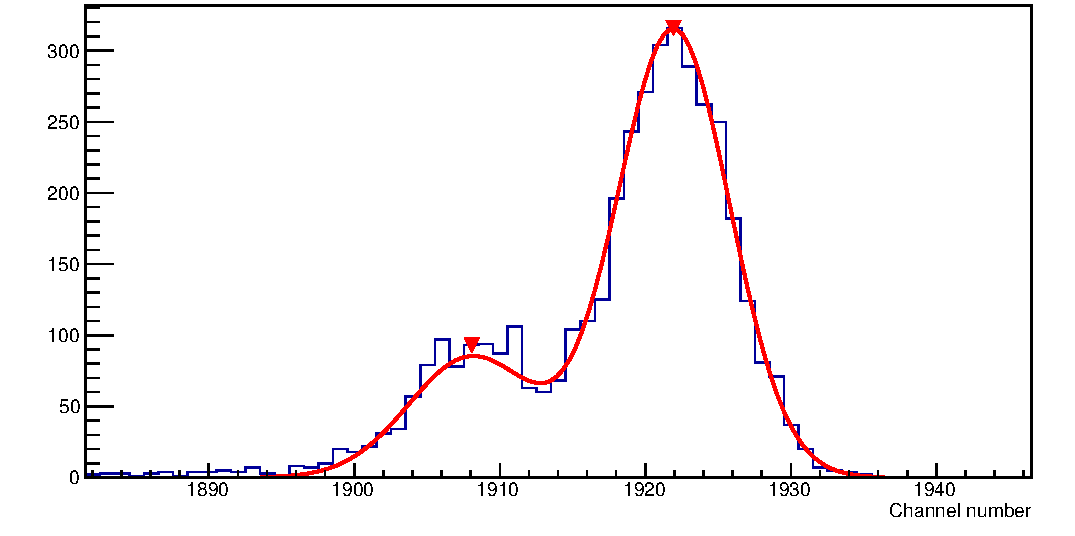
\includegraphics[width=.9\linewidth]{../figures/cali/det1f1PeakMostLeft-cropped}
		\caption{A closer look at the \isotope[244][]{Cm} peak on the above figure. The red line is a fit performed by the \texttt{Calibrator}, and the red triangles indicate the guessed peaks. }
		\label{fig:peakExample}
	\end{subfigure}
	\caption{Calibrations of detector 1}
	\label{fig:CaliExamples}
\end{figure}


\section{Identifying the particles}
After utilizing the AUSAlib tools, the data is ready to be analyzed. Even though the theory dictates that a decay will consist of two \al-particles and one \be-particles, it is not realistic to just assume that each detected event will consist only of this configuration of particles. \\
Therefore we need some cut on what events we will allow through to the analysis. Specifically we are going to impose 3 cuts on the data, a angular cut, a momentum cut and a multiplicity cut.



\subsection{Identifying a hit}
After a hit has been has been detected, and all the relevant information has been extracted from the hit, we can start to analyze what type of particle has hit the detector. 

A important distinction between an \al-particle and a \be-particle is the different interactions with a detector. An \al-particle will be completely stopped by a standard \SI{60}{\mu m} detector, while a \be-particle will pass through it, depositing only a small amount of energy. \\
This is the reason for the SSD's behind each DSSD. The idea is that only a \be-particle will be detected in the SSD's, so if a hit has some energy in a DSSD \textit{and} the corresponding SSD, it will be classified as a \be-particle.\\
\\
This approach however does not work as well as intended. Often what happens is that the thin DSSD will not pick up any energy deposited, and the hit will therefore not be counted. 
But not all of the detectors are \SI{60}{\mu m}. We have two detectors that are around \SI{1000}{\mu m} thick. These detectors are much better at picking up a signal from a \be-particle, so one of the criteria for being a \be-particle in this setup is to have hit either Det2 or DetD.\\

These two criteria are however not enough to uniquely determine that a hit was a \be-particle. We still have to consider the events where a detector has multiple hits. Since a SSD gives no usable information regarding where a particle has hit, we cannot say which particle was a \be-particle and which where a \al-particle. 

Therefore if the \be-particle criteria are true, we mark the particle as a \textit{possible} \be. But since it might as well have been a \al-particle, we also mark it as such.\\
Every hit that does not uphold to the \be-particle criteria are of course marked only as a possible \al-particle.
\\
%When a particle is marked as a \al-particle, we also perform an energy correction, \textcolor{red}{MAYBE ENERGY CORRECTION HERE??}
%
When all the particles have been identified, we impose the first cut to the data. A multiplicity cut that says we need at least two \al-particles. If there are less, we discard the event. 
\\
When we at least have two distinct particles that can be \al-particles, we look at their mutual difference in momentum. The particle pair with the least difference in momentum will be chosen as the only \al-particles that can be present in an event. Then we have assured that every other particle we see in the event, is possible \be-particle candidates. 
\\
When each particle has been identified or discarded, all remaining particle-specific information is stored to the given particle for easy analysis henceforth.

\section{Angular cut}
When \isotope[8][]Be decays, and produces the two \al-particles, it will do so under conservation of momentum. The decay in any direction, but the angle $\theta$ between them will be close to  $180\degree$. Therefore the first cut that we give to the data, is that two of the particles that are \al candidates, must have a mutual angle of close to $180\degree$.\\


On \cref{fig:cosAll} a plot of all the the mutual angles are shown. A quick glance will give that most particles will have mutual angle of close to $180\degree$. 

\begin{figure}[h]
	\centering
	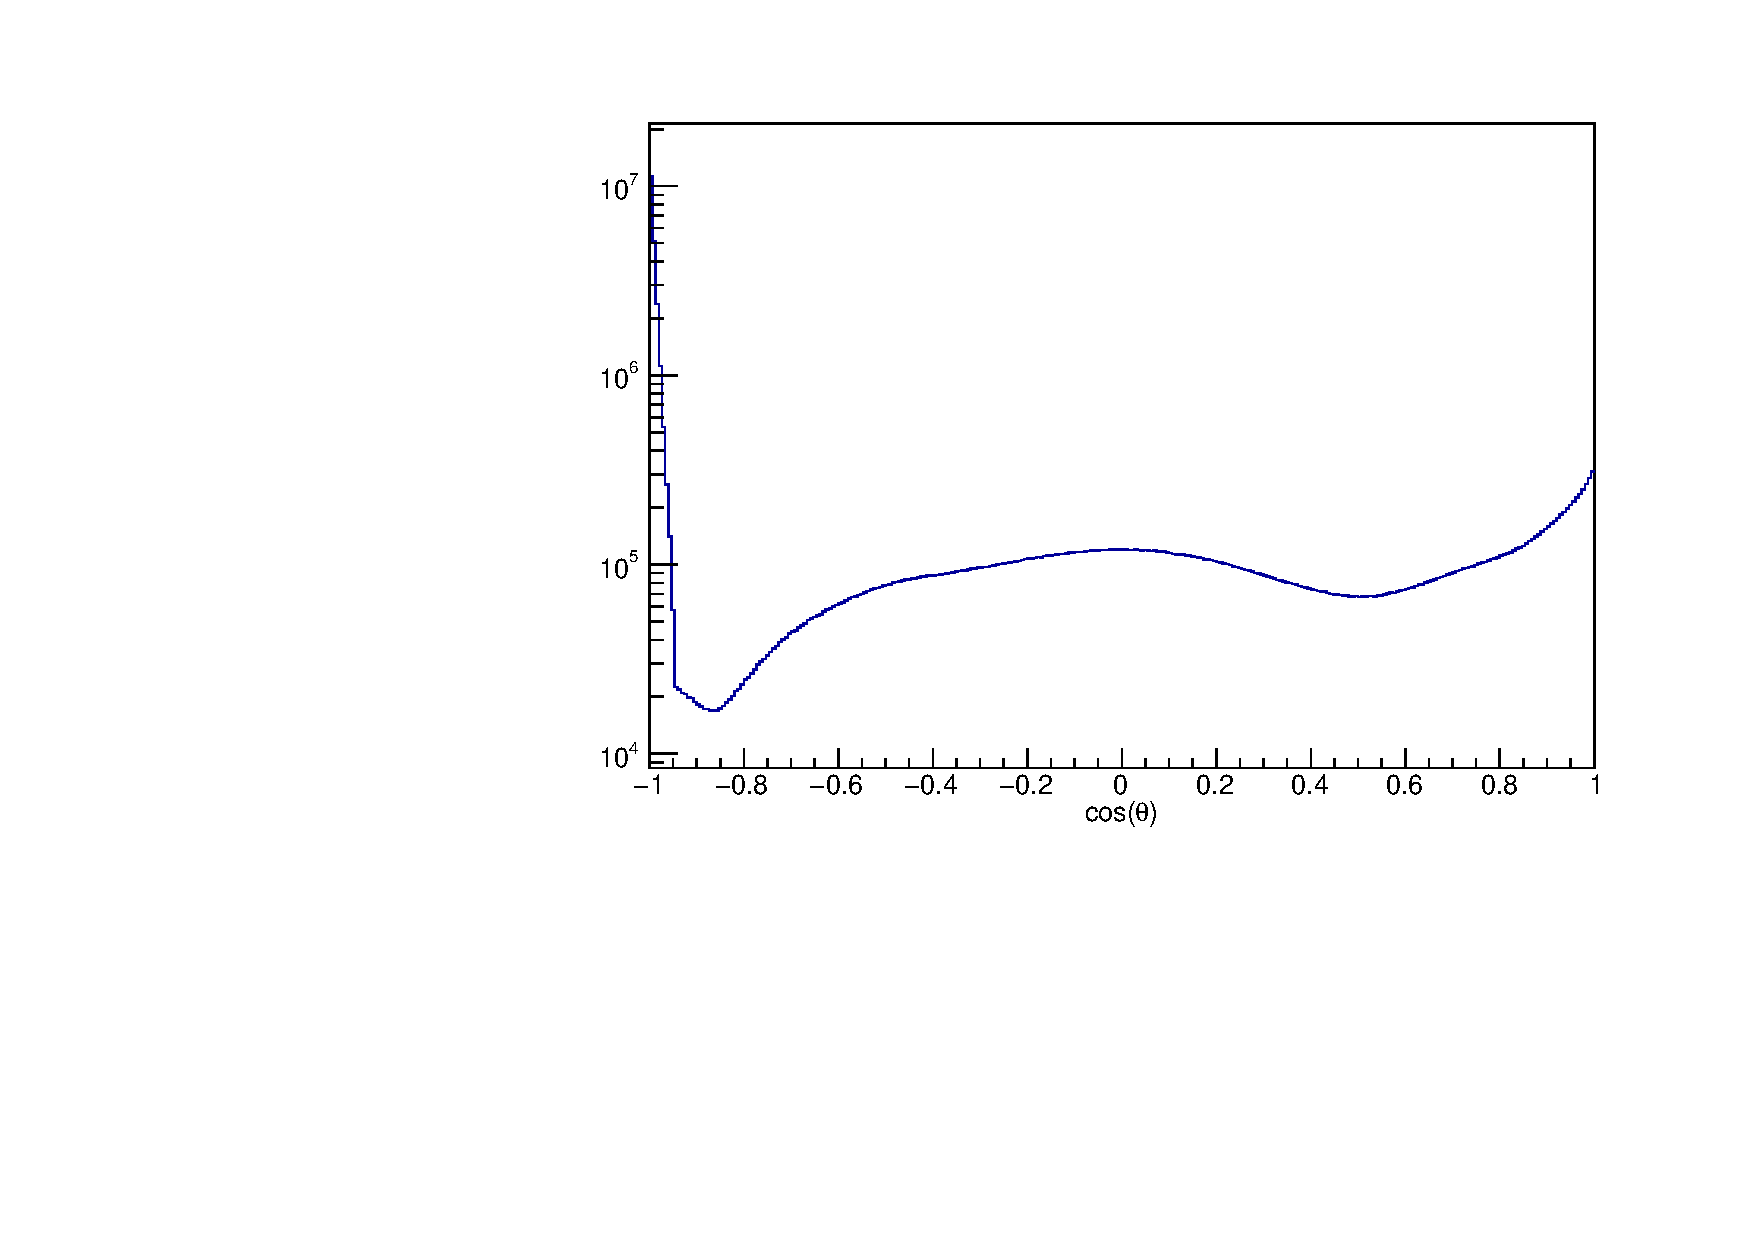
\includegraphics[width=\linewidth]{../figures/cosang.pdf}
	\caption{A histogram of all the mutual angles between all particles.}
	\label{fig:cosAll}
\end{figure}

By looking at this, we see that most of the angles will lie close to $180\degree$, and now we must decide exactly where to do the cutoff. 
By taking a sharp cutoff at $\cos(\theta) \geq -0.99$, we will exclude a great deal of good measurements, on the other hand, a too soft cut will not accomplish anything, as too many "wrong" particles will let through the check. By trying different cuts, we have found that $\cos(\theta) \geq -0.95$ is a good cutoff, and this corresponds to 161\degree. 



\section{Momentum cut}
The second cut we perform on the data is a \textit{total} momentum cut. On \cref{fig:totalMomentum} the total momentum for the two identified \al-particles are shown. 
A prominent peak lies around \SI{13.000}{keV/c}, and ends around \SI{40.000 }{keV/c}. 
We impose a cut of maximum \SI{40}{MeV/c}, as this will include the large amount of pairs lying in the peak, which must be \al-\al pairs. A \al-particle with energy \SI{1500}{keV} will have a momentum of \SI{105}{MeV/c}, and a free electron of \SI{3000}{keV} will have a momentum of \SI{1.7}{MeV/c}. 
The majority of particles lies around these energies, and no matter where the \be-particle will hit, the total momentum is still much larger than the \SI{40}{MeV/c} cutoff. 
\begin{figure}[h]
	\centering
	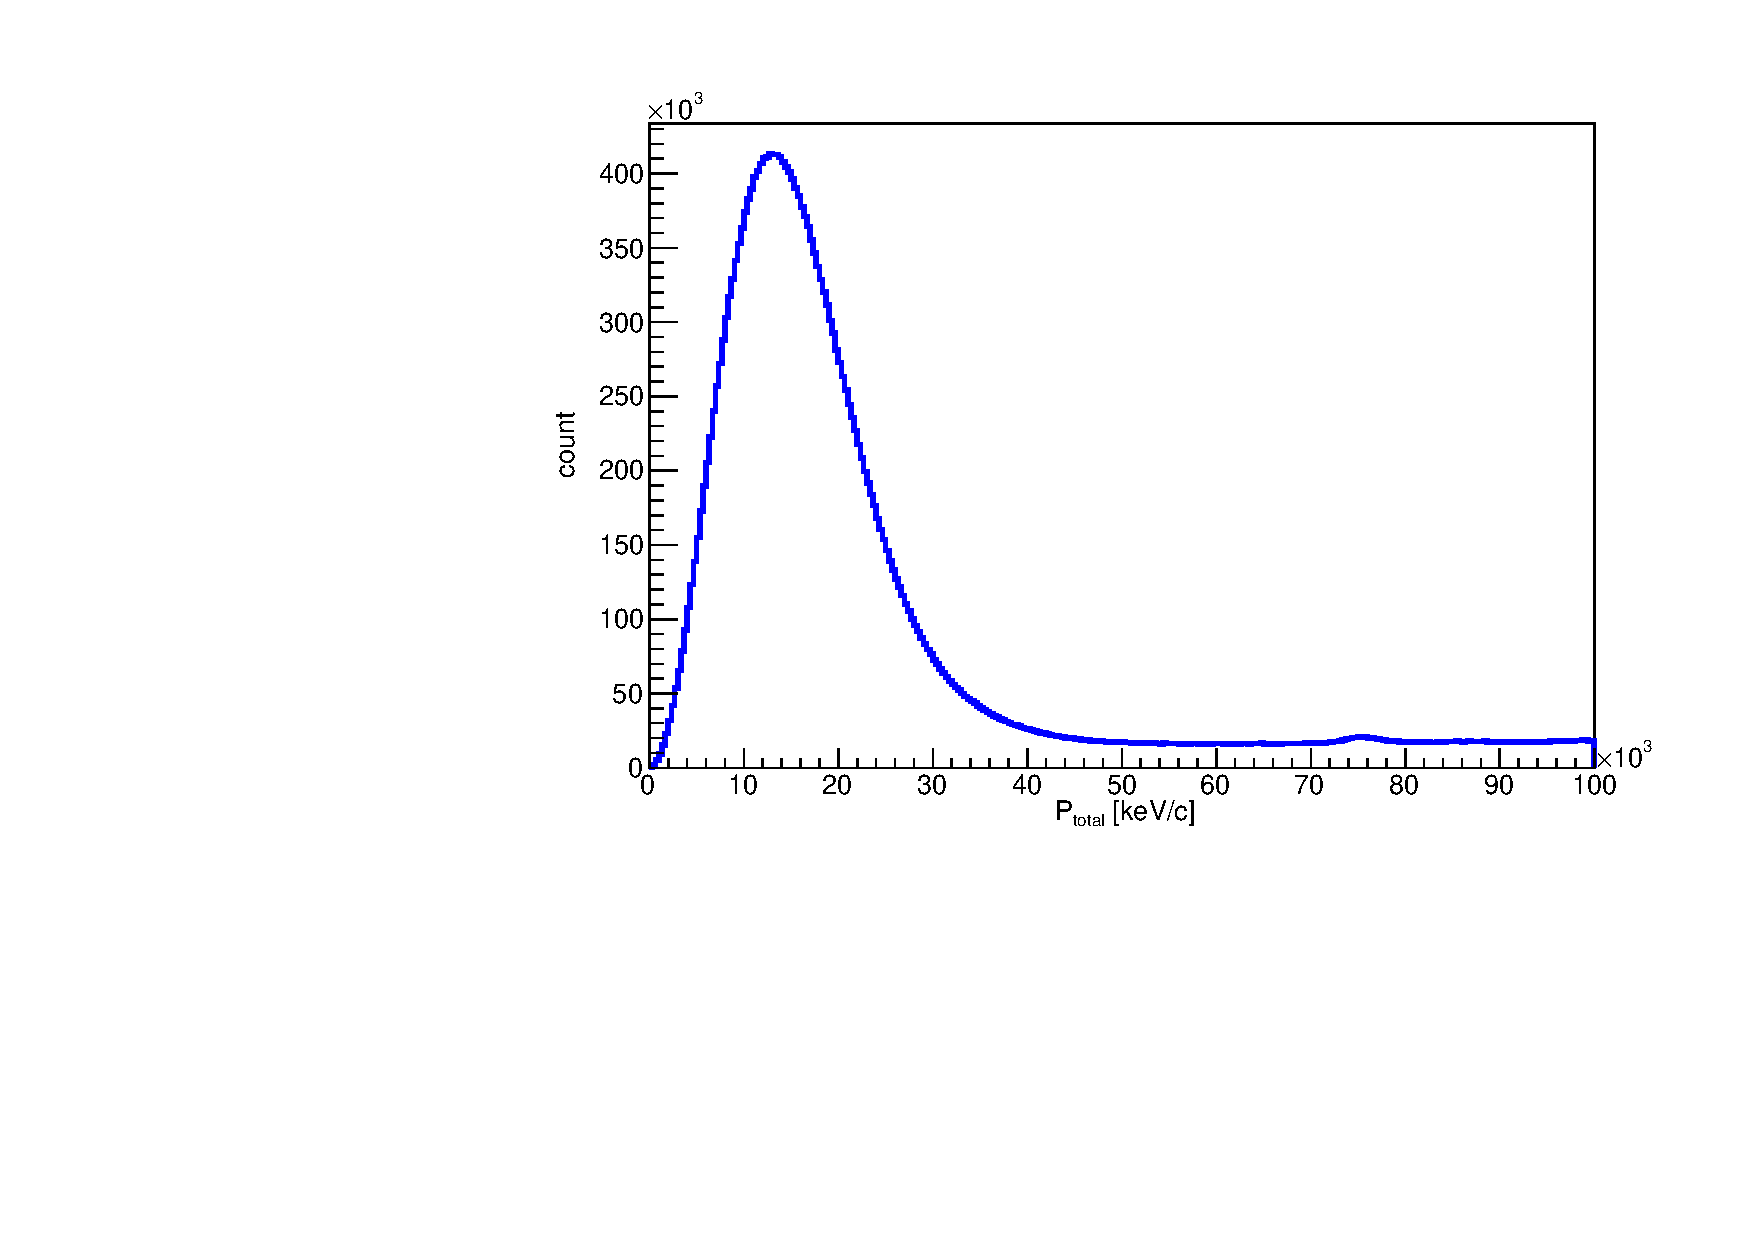
\includegraphics[width=\linewidth]{../figures/ptotNoCut.pdf}
	\caption{The total momentum of the two \al-particles.}
	\label{fig:totalMomentum}
\end{figure}

\section{Multiplicity cut}
The last cut that we want to impose on the data, is a multiplicity cut. This cut is just to ensure that we have the amount of particles that we expect. 
Therefore a hard criteria is that there must be at least two distinctly identified \al-particles. \\

With regards to the \be-particles, we are more loose. Here we say that there must at least be one, but more can occur. This is quite rare, but the we still take that event into account, as the \be-particles should have an isotropic distribution, and therefore should not in any case be affected by the other \al-particles. On \cref{fig:mulBeta} we see the multiplicity of \be-particles, and in most of the events, we have not detected any \be-particles, and when we do, there is a even fewer events with more than one beta. So most of the time, we are in the expected case with two \al-particle and one \be-particle. 

\begin{figure}[h]
	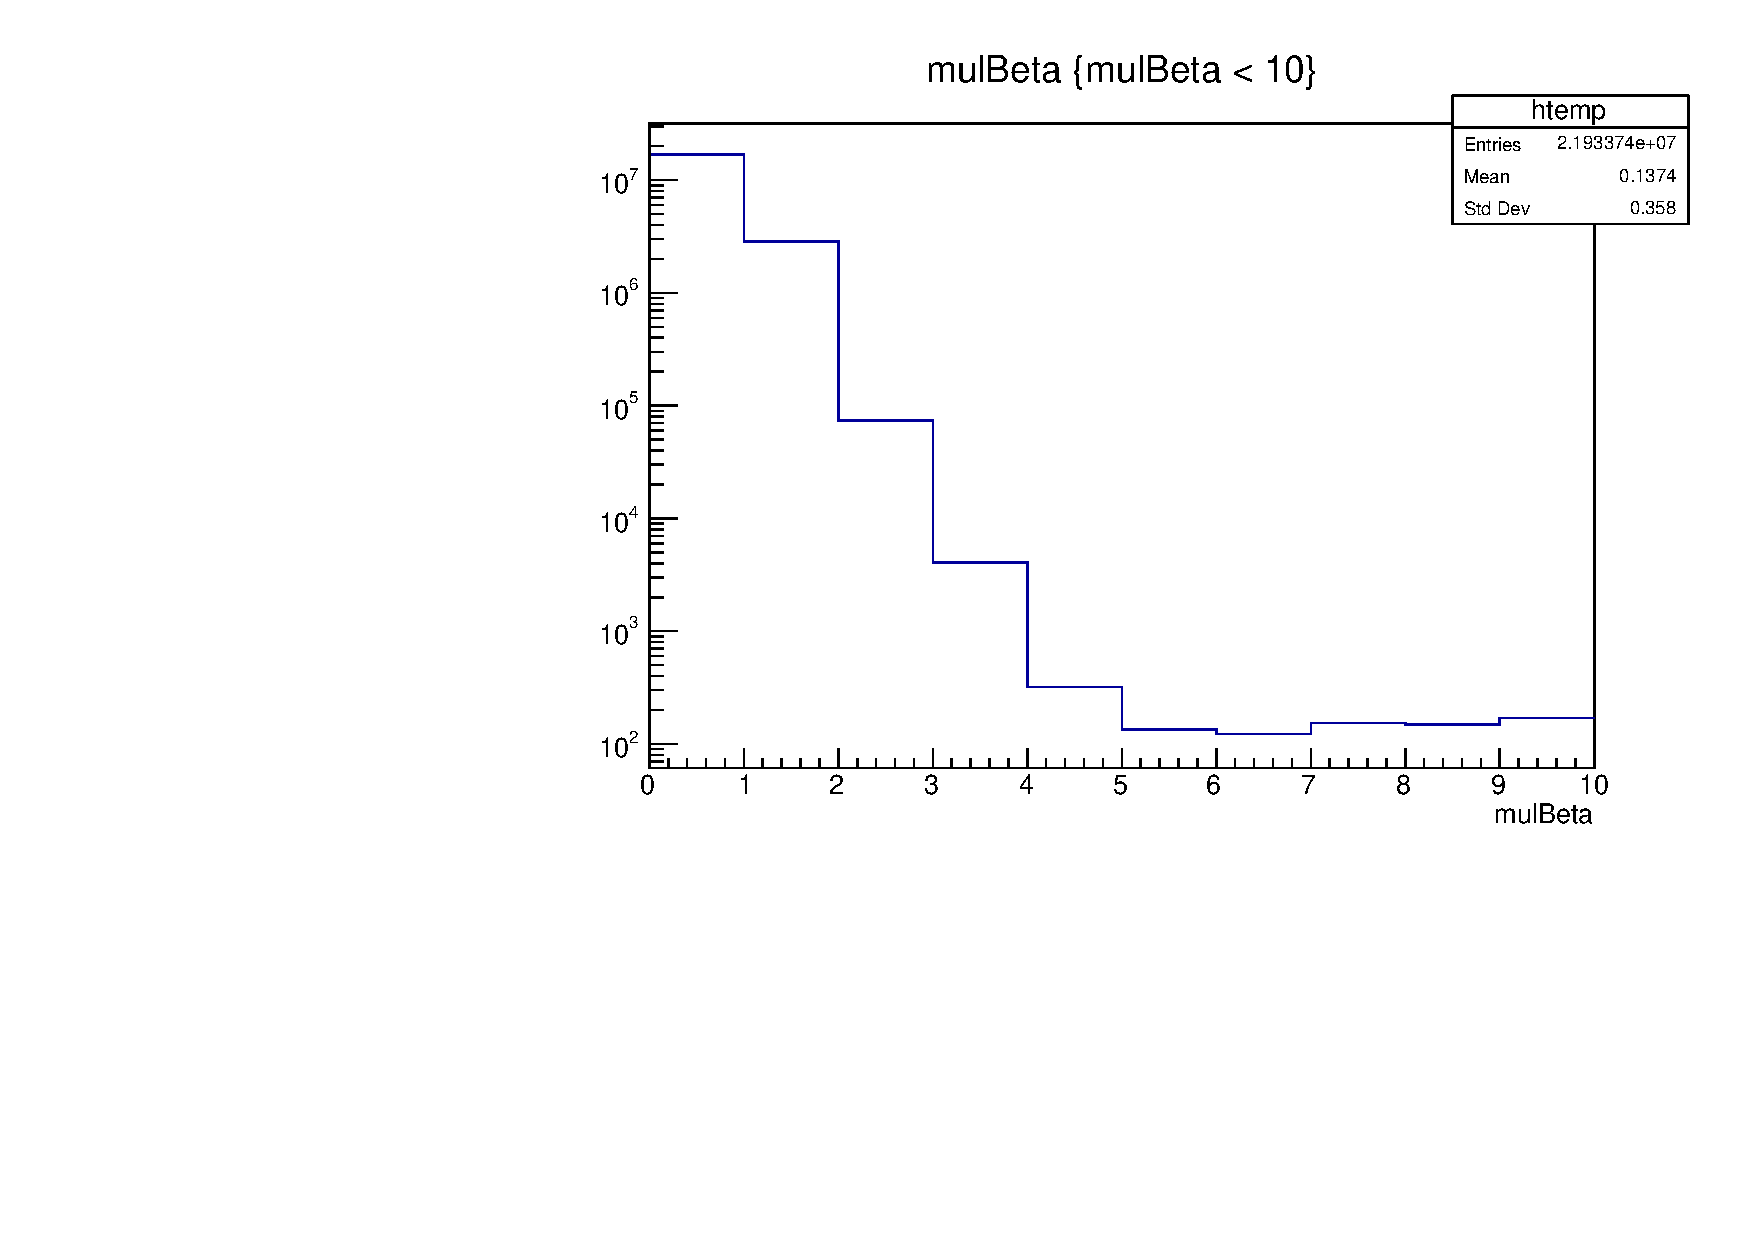
\includegraphics[width=\linewidth]{../figures/mulBeta.pdf}
	\caption{The multiplicity of the \be-particles.}
	\label{fig:mulBeta}
\end{figure}